\RequirePackage[l2tabu, orthodox]{nag}
\documentclass{article}
\usepackage[letterpaper]{geometry}
\usepackage{siunitx}
\usepackage{multicol}
\usepackage{graphicx}
\usepackage{float}
\usepackage{minted}
\usepackage{booktabs}
\usepackage{subcaption}
\usepackage{hyperref}
\usepackage{fontspec}
\usepackage{multirow}

\setmainfont{Noto Serif}
\setmonofont{Source Code Pro}

\usemintedstyle{xcode}
\setminted{fontsize=\footnotesize, linenos=true}

\begin{document}

\begin{titlepage}
    \begin{center}
        \vspace*{1cm}

        \textbf{\Large{Lab 1}}

        \vspace{0.5cm}

        \LARGE{Simple Calculator}
        \vspace{1.5cm}

        Michael Kwok

        \vfill
        \Large{ECE 315 Lab H41\\
            Department of Electrical and Computer Engineering\\
            University of Alberta\\
            25 February 2021}
    \end{center}
\end{titlepage}
\newpage
\tableofcontents
\thispagestyle{empty}
\newpage
\section{Abstract}
The Zybo Z7 is a digital logic and embedded software development platform by Digilent, containing a Zybo 7000 System on a Chip (SoC) that has both a digital logic fabric (Xilinx 7-series FPGA) and a hard processor (ARM Cortex-A9). Extra minor electronic components are also included on the board, such as the push buttons that were used in this lab. The board allows for extension via the PMOD system, which was also used in this lab. The programs all ran on the FreeRTOS operating system which provided features, namely multitasking.

The extensions used were the PMOD SSD, a seven segment display module, and the PMOD KYPD, a 16 character keypad. The seven segment display module was used in the first two parts, to get some practice with the board. In the first part, this was done by getting values input on the keypad to get printed on the seven segment display. In the second part, a simple single digit calculator was to be written, where values input into the keypad were operated by the selected button on the FPGA board.

The final involves the design of a full multi-digit calculator that operated on 32-bit integers, along with overflow detection for certain operations and the ability to calculate a factorial. The seven segment digit display was not used for this part, as there would not be enough space to show the result. Instead, the results were shown via a serial connection to the FPGA board.

All code for this lab has been attached in the Appendix.

\section{Design}
\subsection{Part 1}
A simple ``echo'' program was expected for this part, where values input into the keypad has to be displayed on the seven segment display. Since the goal was simple, we only used a single task to get it done.

A function to convert char values to a bit array for output in the seven segment display was written. The bit array was in the format \verb|0b(c)GFEDCBA| where \verb|c| refers to the Cathode lead and \verb|GFEDCBA| refers to the segments in the seven segment display. The shape and corresponding letters are defined in figure~\ref{fig:ssd_sketch}.

We were also required to set up the GPIO actions for the seven segment display, such as the initial pin setup and the GPIO output. Here, we used the provided Xilinx APIs provided in [1], with functions starting with \verb|XGpio| specifically \verb|XGpio_DiscreteWrite|.

Buttons pressed on the keypad will get shown on both sides of the seven segment display without visible flickering. This was not a given as writing to one side of the display would turn off the other. In the end, the objective was accomplished by swapping which side to flash the digit on very quickly, about \SI{10}{\milli\second} per digit.
\begin{figure}[b]
    \centering
    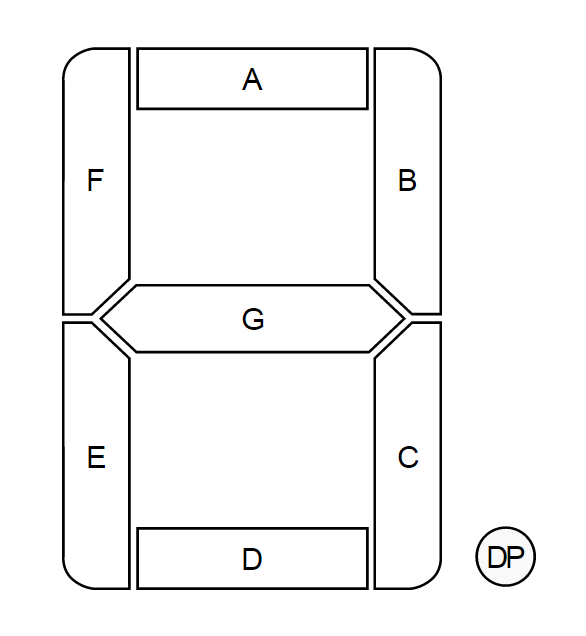
\includegraphics[width=0.2\textwidth]{ssd_sketch.png}
    \caption{Labelled PMOD SSD, Copyright Digilent}
    \label{fig:ssd_sketch}
\end{figure}
\subsection{Part 2}
The objective for this part was to make a single digit calculator program on the board with two concurrent tasks. The first task would be solely handling input, while the second task idles until there are things to calculate and output.

Here we were required to set up the GPIO actions for the seven segment display and the on board buttons. The buttons are set to do addition, subtraction, multiplication and division. Like previously, this was done by using the \verb|XGpio| functions. The push buttons are read with \verb|XGpio_DiscreteRead|

In the transmit task, we had to write the code for reading keypad input, processing it to send through a queue and managing priority levels to allow the receive task to run. The transmit tasks with \verb|xQueueSendToBack|[3] until the queue has 2 items in it, the operands to be operated on together. Once 2 items has been input, the priority of the main task is dropped by 2 with \verb|vTaskPrioritySet|[2], to ensure that the priority is below the receive task.

In the receive task, we receive input from the queue, read the operator value from the push button with \verb|XGpio_DiscreteRead| then calculating the answer. If the answer is less than 0 or if it's a division by zero, it will not get printed on the seven segment display, otherwise the seven segment display will show the desired output. After this is done, the task moves the transmit task higher in terms of priority, with \verb|vTaskPrioritySet| again.

\subsection{Part 3}
Here the goal was to make a calculator that is able to handle 32 bit unsigned inputs and produce a 32 bit output, along with overflow detection for addition and multiplication. Two tasks were used for this, one for input processing and one for calculation and result printing.

Unlike before, we did not use the seven segment display or the board buttons so we did not have to set up \verb|XGpio_DiscreteRead| for either peripheral. All output was to be written out in the serial terminal instead. Similarly to the previous part, we had to manage priority levels in the tasks, so the same code was reused in this part.

The queue set up in this part was of size 3, as we needed to send the requested operation too. The way the operation selection was handled internally was using an enum, to simplify the handling of calculation in the receive task.

\section{Testing}
\begin{table}[H]
    \centering
    \begin{tabular}{lllll}
        \toprule
        Part                    & Description        & Input                          & Output            & Expected Output   \\
        \midrule
        \multirow{4}{*}{Part 2} & Simple Addition    & 1 E 1 E ADD                    & 2                 & 2                 \\
                                & 2 Digit Output     & 9 E 2 E MUL                    & 1 then 8          & 1 then 8          \\
                                & Division by Zero   & 3 E 0 E DIV                    & None              & None              \\
                                & Negative Number    & 2 E 3 E SUB                    & None              & None              \\
        \midrule
        \multirow{3}{*}{Part 3} & Factorial          & 3 F 5 F D                      & \(3! = 6\)        & \(3! = 6\)        \\
                                & Overflow Detection & \(123456789 \times 123456789\) & Overflow detected & Overflow detected \\
                                & Simple addition    & \(100 + 200\)                  & 300               & 300               \\
        \bottomrule
    \end{tabular}
\end{table}
\section{Conclusion}
This lab focused on the ability for different tasks to communicate and the usage of GPIO for input output. The separation of tasks improves modularity, allowing us to focus on getting singular parts to work properly first, and work well in concert. This can be useful in future labs where multiple tasks might be required to be done at the same time. The method used for communication between modules was shared data queues.

\section{References}
\begin{enumerate}
    \item \url{https://xilinx.github.io/embeddedsw.github.io/gpio/doc/html/api/xgpio_8h.html}
    \item \url{https://www.freertos.org/a00129.html}
    \item \url{https://www.freertos.org/xQueueSendToBack.html}
\end{enumerate}
\newpage
\appendix
\section{Part 1}
\inputminted{C}{part1_lab1.c}
\newpage
\section{Part 2}
\inputminted{C}{part2_lab1.c}
\newpage
\section{Part 3}
\inputminted{C}{part3_lab1.c}
\end{document}
